\documentclass{article}
%\usepackage{geometry}
%\geometry{top = 1in, bottom = 1in, left = 1in, right = 1in}
\usepackage[top = 0.7in, bottom = 0.7in, left = 0.7in, right = 0.7in]{geometry}
\usepackage{amsmath,amssymb,amsthm,mathrsfs}
\usepackage{graphicx}
\usepackage{bm}
\usepackage{float}
\usepackage[font=footnotesize,labelfont=bf]{caption}
\usepackage{movie15}
\usepackage{hyperref}

\usepackage{fancyhdr}
\pagestyle{fancy}
\rhead{\footnotesize {07/27/2012 ; MESA version 4161} }
\chead{\footnotesize {Authors: Jared Brooks, Lars Bildsten, Bill Paxton} }
\lhead{\footnotesize {mesa/star/test\_suite/make\_metals} }

\begin{document}
	
	\begin{center}
		\begin{Large}
		       \textbf{MAKE METALS}\\
		\end{Large}
	\end{center}

        This test is to show how to create metals in a star that starts as only hydrogen and helium.  Therefore, this test should be cut off when the mass fraction for central helium drops below $10^{-4}$ (\texttt{xa\_central\_lower\_limit\_species(1) = 'he4' ; xa\_central\_lower\_limit(1) = 1d-4}).\\

        This test case creates a 3 $M_\odot$ pre-main sequence model with uniform composition (mass fractions listed below) and center temperature of $5\times10^5$ K and evolves it for approximately 217 Myr.\\

        \noindent Initial composition (mass fractions):
        \begin{itemize}
                \item $^1$H: 0.75
                \item $^4$He: 0.25
        \end{itemize}

        Below we can see the evolution track the star takes in the HR-diagram (figure \ref{fig:1}) from a pre-main sequence star to an AGB star.  To the right is a plot of the evolution of the burning luminosities near the end of the run (figure \ref{fig:2}).  This shows the PP burning was dominant for the majority of the stars life, until CNO and triple alpha burning overtake PP burning.

        \begin{figure}[H]
                \begin{minipage}[b]{0.5\linewidth}
		       \centering
		       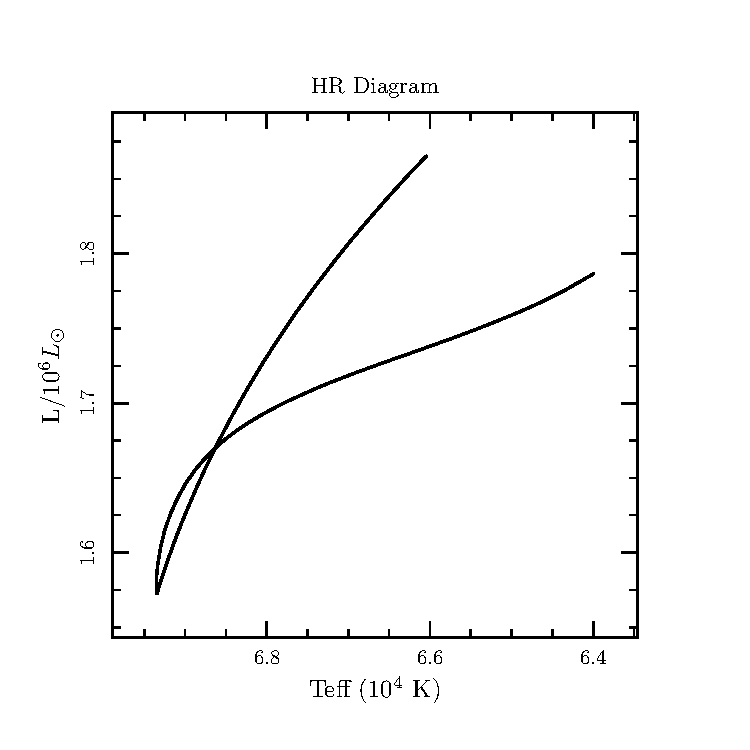
\includegraphics[width = 3.8in]{/Users/jaredbrooks/make_metals/plots_out/HR_Diagram.pdf}
		       \caption{HR-diagram}
		       \label{fig:1}
                \end{minipage}
                \hspace{0cm}
                \begin{minipage}[b]{0.5\linewidth}
                       \centering
                       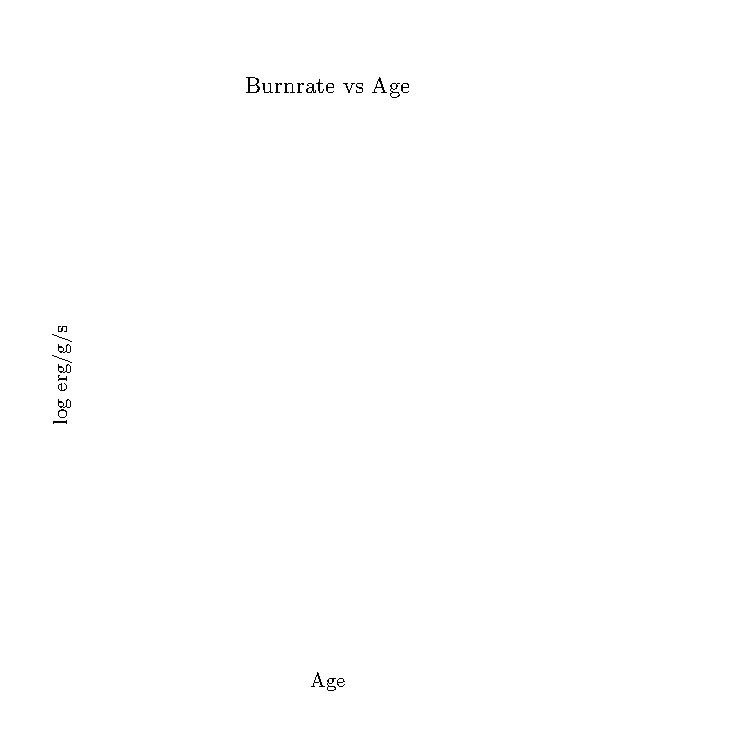
\includegraphics[width = 3.8in]{/Users/jaredbrooks/make_metals/plots_out/Burnrate_vs_Age.pdf}
                       \caption{Burning luminosities show CNO and triple alpha overtaking PP}
                       \label{fig:2}
                \end{minipage}
	\end{figure}

        \pagebreak

        The plot of burning rates vs q, where q is the fraction of star mass interior to outer boundary of each zone, moving outwards from the core, taken at the end of the run (figure \ref{fig:3}) shows that this is an AGB star engaged in double shell burning. To the right is a plot of the evolution of the star's center temperature vs center density (figure \ref{fig:4}).

        \begin{figure}[H]
                \begin{minipage}[b]{0.5\linewidth}
                       \centering
                       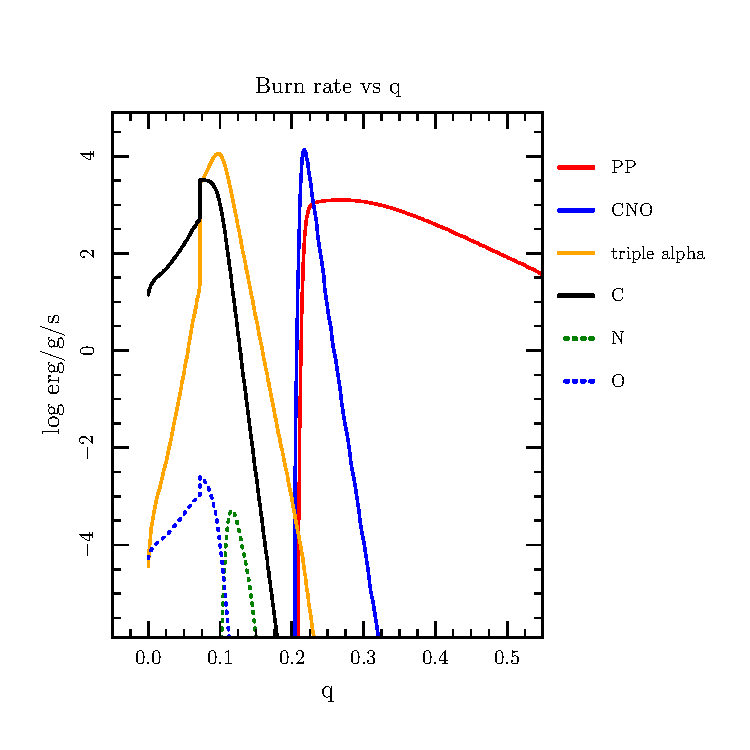
\includegraphics[width = 3.8in]{/Users/jaredbrooks/make_metals/plots_out/Burnrate_vs_q_finish.pdf}
                       \caption{Burning rate profile shows double shell burning}
                       \label{fig:3}
                \end{minipage}
                \hspace{0cm}
                \begin{minipage}[b]{0.5\linewidth}
                       \centering
                       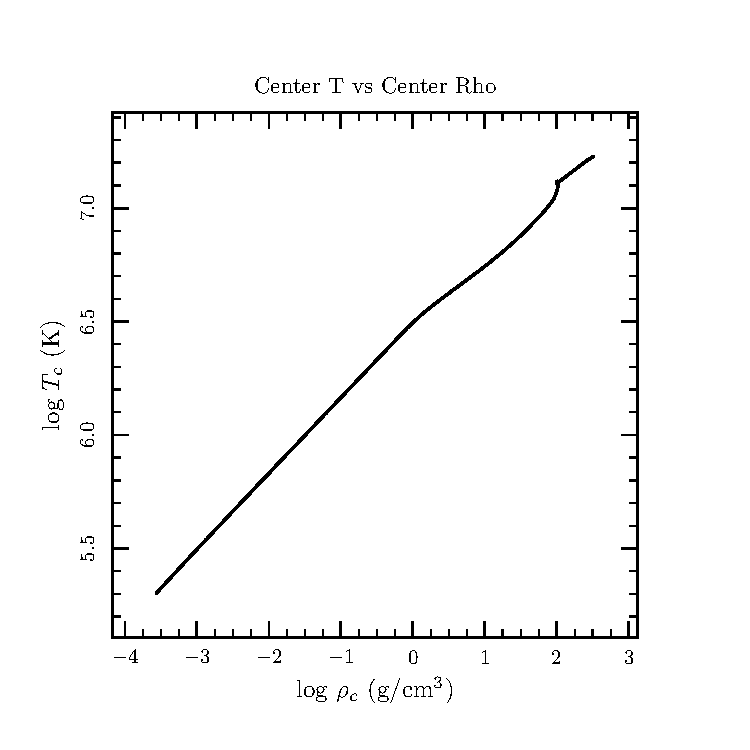
\includegraphics[width = 3.8in]{/Users/jaredbrooks/make_metals/plots_out/Tc_vs_Rhoc.pdf}
                       \caption{Center temperature vs center density}
                       \label{fig:4}
                \end{minipage}
        \end{figure}

        \pagebreak

        Below is a video showing changes in mass fractions of elements plotted against m/$M_\odot$.  The number at the top-right is the model number.  Click the figure to begin the video, double click to replay (must be using adobe reader to view movie).  Below that is an abundance profile taken at the end of the run (figure \ref{fig:5}) to show what elements were consumed and what elements were produced.  (Note: The Ne20 shown here actually represents Ne22, this is because \texttt{MESA} is using a simplified nuclear reaction network.)

        \begin{figure}[H]
          \includemovie[poster,text={\small(Loading Video...)}]{18cm}{15cm}{abun.mp4}
        \end{figure}

        \begin{figure}[H]
                \centering
                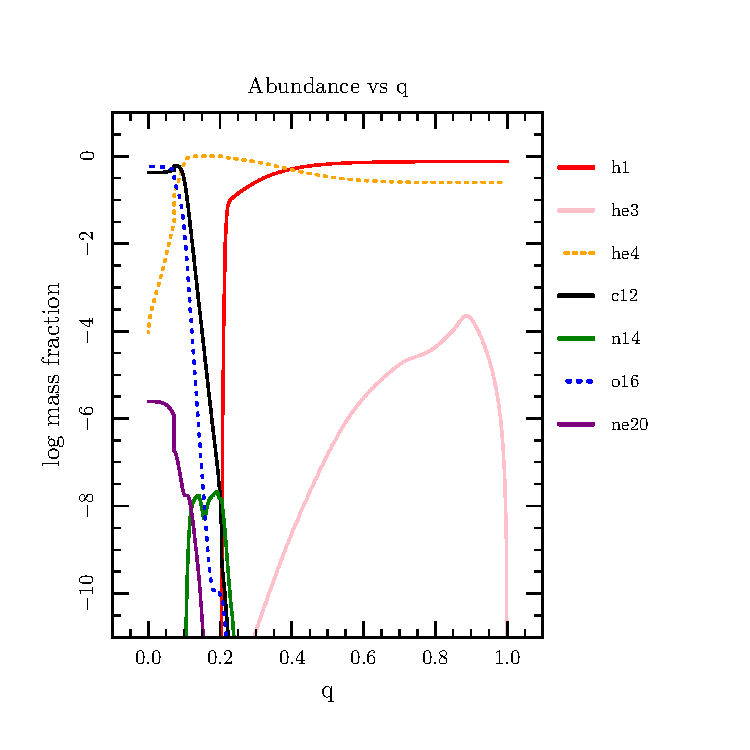
\includegraphics[width = 5in]{/Users/jaredbrooks/make_metals/plots_out/Abundance_vs_q_18.pdf}
                \caption{Abundance profile at end of run}
                \label{fig:5}
        \end{figure}

        \pagebreak

        This final plot (figure \ref{fig:7}) is meant to show a few internal \texttt{MESA} variables, such as the size of the time-step, the number of zones, and the number of retries against the model number in order to give some understanding of how hard \texttt{MESA} is working throughout the run and where some areas of problems/interest might be.

        \begin{figure}[H]
                \centering
                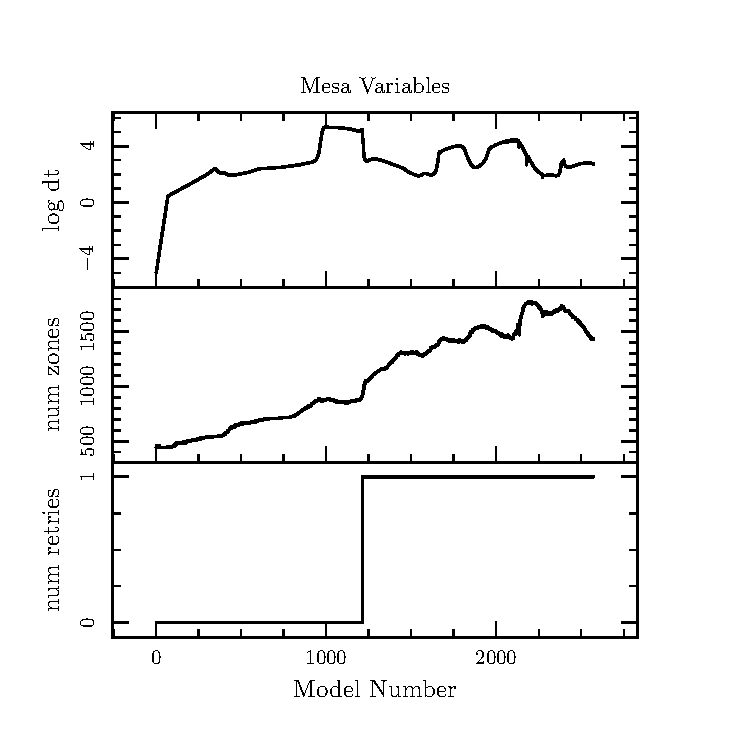
\includegraphics[width = 5in]{/Users/jaredbrooks/make_metals/plots_out/Mesa_Variables.pdf}
                \caption{\texttt{MESA} variables plotted against model number show how hard \texttt{MESA} is working}
                \label{fig:7}
        \end{figure}

\end{document}
